% Fig. 4.1 -- 二項 pmf 的形狀隨 p 變化，三個面板。
% 書稿來源: mathstatch4.tex 第 209 至 289 行，其中三個 tikzpicture 落在第 211、238、265
%   行，各包在一個 .33\textwidth 的 minipage 內，書稿橫排成一列。三個面板都以 pgfplots 的
%   \addplot[only marks] 畫 n = 10 的二項機率函數，取樣點 x = 0, 1, ..., 10，scale = 0.7;
%   只畫 x 軸 (axis x line=center)，y 軸不畫 (axis y line=none) 也不顯示刻度數值，
%   兩軸皆不寫軸名，xmin = -0.5、xmax = 11、ymin = -0.01，ymax 依序為 0.4、0.3、0.4，
%   三者各以 \addlegendentry 標出 B(10,0.2)、B(10,0.5)、B(10,0.8)。
%
% 機率值一律預先算出後寫死 (六位小數)，不在圖檔內以階乘求值，避免 pgfmath 的定點運算
% 在 10! 這一級距上失去精度:
%   p = 0.2  0.107374 0.268435 0.301990 0.201327 0.088080 0.026424 0.005505
%            0.000786 0.000074 0.000004 0.000000
%   p = 0.5  0.000977 0.009766 0.043945 0.117188 0.205078 0.246094 0.205078
%            0.117188 0.043945 0.009766 0.000977
%   p = 0.8  即 p = 0.2 那一列左右翻轉。
%
% 對書稿的四處調整:
%
%   1. 三個面板改為上下堆疊。書稿並排成一列，在網頁上每個面板只分到約 110 px，
%      面板下方的標示比面板本身還寬。作法同 sum-range-two-cases.tex。
%   2. y 軸上界依書稿保留 0.4 / 0.3 / 0.4 不統一 (見候選稿內的 fig-pending 註記)，
%      作法是各面板自訂 y 單位: 上下兩個面板 2.2cm / 0.4 = 5.5cm，中間面板
%      2.2cm / 0.3 = 7.3333cm。三個面板的繪圖高度因而相同，與書稿的成像一致。
%   3. 書稿的 \addlegendentry 圖例框改為各面板下方一行標示，記號依網頁體例寫
%      \mathrm{Bin}(10, p)，與 binomial-distribution.md 內文一致。
%   4. x 軸末端補上軸名 $x$ (書稿 xlabel 為空)。刻度畫在每一個整數，刻度數值只標
%      0、2、4、6、8、10; 每一個整數都標的話相鄰標籤只差 0.62cm，不足
%      CH2_FIGURE_SPECS.md 1.3 所定的 0.6cm 下限的餘裕。
%
% 版面: x = 0.62cm，繪圖範圍自 x = -0.7 到 x = 11.0 再加軸名，原生寬約 7.9cm，
%   在 CH2_FIGURE_SPECS.md 1.3 的 9.0cm 上限之內。圖內沒有下標，最小字即 10pt 本文級。
%
% 產製:
%   pdflatex binomial-pmf-shapes.tex
%   pdftocairo -svg binomial-pmf-shapes.pdf ../../images/teaching-topics/binomial-pmf-shapes.svg

\documentclass[tikz,border=2pt]{standalone}
\usepackage{amsmath}
\usepackage{amssymb}
\usepackage{xcolor}
\usetikzlibrary{arrows.meta}

\definecolor{journalink}{HTML}{1F1C18}
\definecolor{journalmuted}{HTML}{8A7F72}
\definecolor{journalaccent}{HTML}{9C2D2D}

\begin{document}
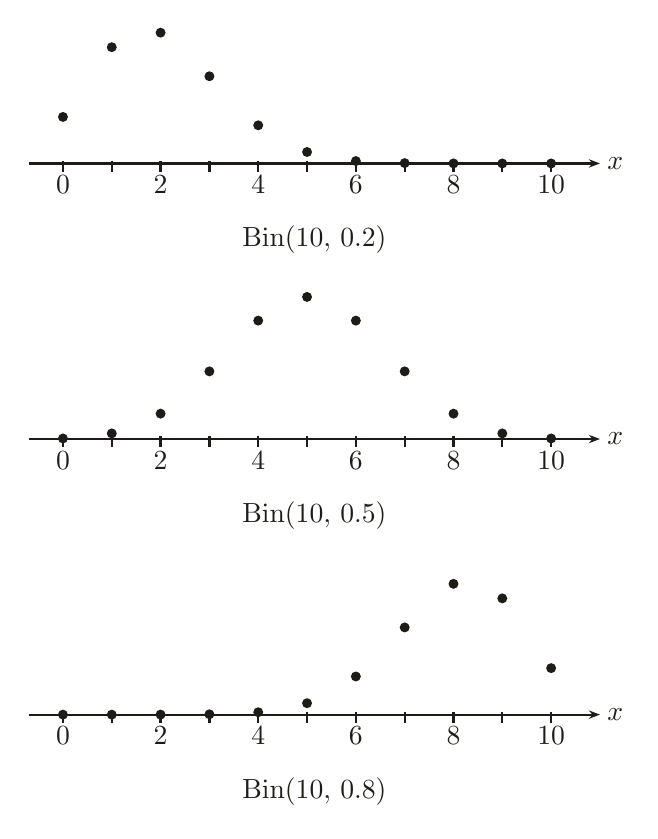
\begin{tikzpicture}[
  x=0.62cm,
  every node/.style={font=\normalsize, journalink},
  axis/.style={journalink, line width=0.8pt, -{Stealth[length=4pt]}},
  tick/.style={journalink, line width=0.8pt},
  mass/.style={circle, fill=journalink, inner sep=0pt, minimum size=3.6pt}
]

%% ==== 上面板: p = 0.2，右偏 =========================================
\begin{scope}[y=5.5cm]

  \draw[axis] (-0.7,0) -- (11.0,0);
  \node[anchor=west, inner sep=2.5pt] at (11.0,0) {$x$};

  \foreach \k in {0,...,10}
    \draw[tick] ([yshift=1pt]\k,0) -- ([yshift=-3pt]\k,0);
  \foreach \k in {0,2,4,6,8,10}
    \node[anchor=north, inner sep=2pt] at ([yshift=-0.08cm]\k,0) {$\k$};

  \foreach \k/\p in {0/0.107374, 1/0.268435, 2/0.301990, 3/0.201327,
                     4/0.088080, 5/0.026424, 6/0.005505, 7/0.000786,
                     8/0.000074, 9/0.000004, 10/0.000000}
    \node[mass] at (\k,\p) {};

  \node[anchor=north, inner sep=2pt] at ([yshift=-0.72cm]5.15,0)
    {$\mathrm{Bin}(10,\,0.2)$};

\end{scope}

%% ==== 中面板: p = 0.5，對稱 =========================================
\begin{scope}[y=7.3333cm, yshift=-3.5cm]

  \draw[axis] (-0.7,0) -- (11.0,0);
  \node[anchor=west, inner sep=2.5pt] at (11.0,0) {$x$};

  \foreach \k in {0,...,10}
    \draw[tick] ([yshift=1pt]\k,0) -- ([yshift=-3pt]\k,0);
  \foreach \k in {0,2,4,6,8,10}
    \node[anchor=north, inner sep=2pt] at ([yshift=-0.08cm]\k,0) {$\k$};

  \foreach \k/\p in {0/0.000977, 1/0.009766, 2/0.043945, 3/0.117188,
                     4/0.205078, 5/0.246094, 6/0.205078, 7/0.117188,
                     8/0.043945, 9/0.009766, 10/0.000977}
    \node[mass] at (\k,\p) {};

  \node[anchor=north, inner sep=2pt] at ([yshift=-0.72cm]5.15,0)
    {$\mathrm{Bin}(10,\,0.5)$};

\end{scope}

%% ==== 下面板: p = 0.8，左偏 =========================================
\begin{scope}[y=5.5cm, yshift=-7.0cm]

  \draw[axis] (-0.7,0) -- (11.0,0);
  \node[anchor=west, inner sep=2.5pt] at (11.0,0) {$x$};

  \foreach \k in {0,...,10}
    \draw[tick] ([yshift=1pt]\k,0) -- ([yshift=-3pt]\k,0);
  \foreach \k in {0,2,4,6,8,10}
    \node[anchor=north, inner sep=2pt] at ([yshift=-0.08cm]\k,0) {$\k$};

  \foreach \k/\p in {0/0.000000, 1/0.000004, 2/0.000074, 3/0.000786,
                     4/0.005505, 5/0.026424, 6/0.088080, 7/0.201327,
                     8/0.301990, 9/0.268435, 10/0.107374}
    \node[mass] at (\k,\p) {};

  \node[anchor=north, inner sep=2pt] at ([yshift=-0.72cm]5.15,0)
    {$\mathrm{Bin}(10,\,0.8)$};

\end{scope}

\end{tikzpicture}
\end{document}
